\documentclass[11pt]{exam}
\printanswers
% \documentclass[a4paper,10pt]{article}
\usepackage{tikz}
\usetikzlibrary{arrows,positioning,shapes.geometric}
\usepackage{amsmath,amssymb,complexity}
\usepackage{datetime,enumerate,palatino}
\usepackage{setspace}

\usepackage[utf8]{inputenc}
\usepackage[numbers]{natbib}
\usepackage{mathpartir}
\usepackage{mathtools}
\usepackage{mathpartir}
\usepackage{stmaryrd}
\usepackage{amsfonts}
\usepackage{amsmath}
\usepackage{amsthm}
\usepackage{listings}
\usepackage{multirow}
\usepackage[T1]{fontenc}
\usepackage{helvet}
\usepackage{array}
\usepackage{ragged2e}
\usepackage{tfrupee}  

\textwidth6in

\setlength{\topmargin}{0in} \addtolength{\topmargin}{-\headheight}
\addtolength{\topmargin}{-\headsep}

\setlength{\oddsidemargin}{0in}

\oddsidemargin  0.2in \evensidemargin 0.0in %\parindent0em


\newtheorem{theorem}{Theorem}
\newtheorem{lemma}{Lemma}
\newtheorem{corollary}{Corollary}
\newcommand\tab[1][1cm]{\hspace*{#1}}

%opening
\title{Your Name\\ Your ID}
\author{}
\date{}
\begin{document}

\hrule
\vspace{3mm}
\noindent
{\sf CS6190: Recent Developments in Theoretical Computer Science  \hfill Assignment \#2}
\vspace{3mm}
\noindent
% {\sf Topic: OFWs and PRGs\hfill Due on : $29^{th}$ Dec, 2020}
% \vspace{3mm}
%\hrule

% uncomment the lines below and fill name and roll number of teammates here

%\vspace{3mm}
\noindent
{\sf Roll No: CS14B043\hfill Full Name: Harshal Gawai} 
\vspace{3mm}
\hrule
%%%%%%%%%       1       %%%%%%%%%
\begin{questions}
\question Assuming ETH, show that Vertex Cover does not admit an algorithm running in time $2^{o(n+m)}$ , where $n$ and $m$ are the number of vertices and edges in the input graph, respectively.
\begin{solution}
    Let girth of Graph G be $d$\\
    \pmb{Proof}:\\
    We reduce from Vertex Cover , which is known to admit no $2^{o(n)}$-time algorithm (assuming ETH here)\\
    Lets assume that $d$ is even; otherwise, increase $d$ by one.\\
    Given a vertex cover instance $(G = (V, E), k)$ the reduction is simply to replace each edge $\{u,v\}$ of $G$ by a path on $d$ vertices and to make one endpoint of this path adjacent to $u$ and the other one adjacent to $v$. \\
    Equivalently, subdivide each edge $d$ times.\\
    Let $G'$ denote the resulting graph, and call the paths that are added during the construction the d-paths of $G'$.\\
    
    To complete the construction, set $k':= k + (d/2) \cdot |E(G)|$.\\
    (*we will show, the two instances are equivalent.)\\
    Assume for now that equivalence holds. \\
    The shortest cycle in $G'$ clearly contains more than $d$ vertices \\
    (in fact it contains more than $3d$ vertices).\\
    Moreover, the construction does not increase the maximum degree of $G$, hence $G'$ has maximum degree three, and each original edge was replaced by a path, hence $G$ is 2-degenerate.\\
    Finally, $G'$ has $O(|V(G)|)$ many vertices and edges since $d$ is a constant.\\
    
    Thus, any algorithm that solves $(G', k')$ in $2^{o(|V (G')|+|E(G')|)}$ time can be used to obtain an algorithm that solves Vertex Cover in $2^{o(n+m)}$ time which contradicts the ETH.\\
    To complete the proof it thus remains to show equivalence of the instances.\\
    $(G, k)$ is a yes-instance $\Leftrightarrow$ $(G', k')$ is yes-instance.\\
    
    $(\implies)$Let S be a size-k vertex cover of $G$. Consider the graph $G'-S$.\\
    By construction, all remaining edges are incident with vertices in d-paths. \\
    Moreover, for each d-path, the nonpath neighbor of at least one of its endpoints is contained in $S$ since $S$ is a vertex cover.\\
    Thus, deleting the other endpoint of the path and then every other vertex of the path gives a set of $d/2$ vertex deletions that together destroy all edges that are incident with vertices of this path. \\
    This can be done for all $|E(G)|$ many d-paths, resulting in $(d/2) \cdot |E(G)|$ vertex deletions.\\
    Consequently, $(d/2) · |E(G)| + k$ vertex deletions suffice to destroy all edges in $G'$.\\
    $(\Leftarrow)$\\
    Observe that any vertex cover contains at least $(d/2) · |E(G)|$ vertices that are on d-paths.\\
    Moreover, there is a minimum-cardinality vertex cover such that no two neighbors $u$ and $v$ in a d-path are deleted: Deleting $u$ makes $v$ a degree-one vertex which means that deleting the other neighbor of $v$ instead of $v$ gives a vertex cover which is at most as large as one that deletes $u$ and $v$.\\
    Thus, there is a minimum-cardinality vertex cover $S'$ that contains for each d-path exactly one of its two endpoints.\\
    Moreover, the neighbor of the other endpoint that is not in the d-path is contained in $S'$.\\
    Let $S := S' \cap V$ denote the vertices from $V$ that are contained in $S$.\\
    For each edge $\{u,v\} \in E$, there is a d-path connecting $u$ and $v$ in $E$.\\
    By the discussion above, either $u$ or $v$ is in $S$.\\
    Thus, $S$ is a vertex cover.\\
    Since $S'$ contains at least $(d/2) \cdot |E(G)|$ vertices from d-paths, we have $|S|\leq k$.
\end{solution}

%%%%%%%%%       2       %%%%%%%%%
\question Design an algorithm for Closest String running in time $\mathcal{O} * ((d + 1)^d )$. Formally argue the correctness of the algorithm and the claimed running time bound. (You may assume the simplification to the problem that we discussed in the class.)
\begin{solution}
    Closest String Algorithm:\\\\
    \pmb{Input:} A Closest String instance with a set of \pmb{S} $n$ strings of length $l$, parameters $\vartriangle d$, $d$ and $k$, and a candidate string $x$.\\\\
    \pmb{Output:} A string $s*$ if there exists a set \pmb{S} of at least $n*$ strings where each string in $S$ has distance at most $d$ from $s*$, and “Not found” otherwise.\\
    \pmb{Closest String Algorithm:}
    \begin{enumerate}
        \item If $\vartriangle d < 0$ or $k < 0$ then return “Not found”.
        \item Choose $i \in \{1,…, n\}$ such that $d(x, s_i) > d$. If no such $i$ exists return $x$.
        \item $s_{ret} =$ Closest String Algorithm$(S\setminus \{s_i\}, \vartriangle d, k - 1, x)$. 
        \item If $s_{ret} =$ “not found ” then:
        \begin{enumerate}
            \item $\pmb{P} = \{p \:|\; x[p] \neq s_i [p]\}$;
            \item Choose any \pmb{P'} from \pmb{P} with $|\pmb{P}'| = d + 1$.
            \item For each position $p \in \pmb{P}'$
            \begin{itemize}
                \item Let $x$ be equal to $s_i$ at position $p$.
                \item $s_{ret} =$Closest String  Algorithm$(S, \vartriangle{d - 1}, k, x$).
                \item If $s_{ret} \neq$ “not found”, then return $s_{ret}$ .
            \end{itemize}
        \end{enumerate}
        \item Return “not found”.
    \end{enumerate}
    
    The Algorithm begins with $s_1$ as the candidate center string. If $s_1$ is a center string with respect to $S$ then we are done; otherwise there exists a string $s_1$ that has distance at least $d + 1$ from $s_1$. We “guess” whether $s_1$ belongs in the set of outliers. If it is an outlier then we remove it from $S$ and recurse on the smaller set with $k – 1$. If it is not an outlier then we use $s_1$ to move the candidate string $x$ closer to toward $s_1$.\\\\
    Next lets show that Algorithm is fixed parameter tractable if $d$ and $k$ are parameters.\\
    In the algorithm at each recursive step a string $s$ is selected that has Hamming distance at least $d + 1$ away from the current candidate center string $x$ if one exists; otherwise $x$ is returned since it is a center string.\\
    Then for any $d + 1$ positions where $x$ and $s$ disagree, there is at least one position at which $s$ is equal to the final solution.\\
    The algorithm tries each of the $d + 1$ positions, changes $x$ to $s$ at one of the $d + 1$ the position, reduces $\vartriangle d$ by one, and calls itself recursively.\\
    Hence, $\vartriangle d$ is the current degeneracy parameter at a particular recursive iteration and $x$ is the current candidate center string.\\
    Since the recursion stops after at most d steps the size of the search tree is bounded by $O((d + 1)^d)$.

    
\end{solution}

%%%%%%%%%       3       %%%%%%%%%
\question The conjecture Randomized ETH is similar to ETH, except that in the definition of $\delta_3$ from Conjecture 14.1 in the book, the term “algorithm” is replaced by “randomized algorithm”.  Show that assuming Theorem 14.13, an $\mathcal{O} * (2^{o(k log k)} )$ algorithm for $k * k$ Permutation Clique contradicts Randomized ETH.

%%%%%%%%%       4       %%%%%%%%%
\question For $n \in N$ and $n \geq 3$, the cycle $C_n$ is a graph with vertex set $V(C_n ) = \{v_1 , v_2 , ... , v_n \}$ (all elements distinct) and edge set $E(C_n ) = \{\{v_i , v_(i+1) \} | i \in \{1, 2, ⋯ , n − 1\}\} \cup \{\{v_1 , v_n \}\}$. Show that for each $n \geq 3$, the treewidth of $C_n$ is exactly $2$.
\begin{solution}\\
    \pmb{Given}:\\The cycle $C_n$ is a graph with vertex set $V(C_n ) = \{v_1 , v_2 , ... , v_n \}$\\
    And, edge set $E(C_n ) = \{\{v_i , v_(i+1) \} | i \in \{1, 2, ⋯ , n − 1\}\} \cup \{\{v_1 , v_n \}\}$.\\\\
    First Lets prove that \hspace{1cm}$TW(C)\leq 2$:\\
    we define a tree $T$ , \\
    where\hspace{3.4cm} $V (T ) = \{1, . . . , n-2\}$\\
    and, \hspace{3.6cm} $E(T ) = \{\{i,i+1\} : 1 \leq i \leq n-3\}$\\
    and the family, \hspace{1.9cm}$\mathcal{X} = (X_t, t \in V (T))$\\
    where, \hspace{3.2cm} $X_t = \{v_1, vt+1, v_{t+2}\}$ \hspace{1cm}for any vertex $t \in V(T)$\\\\
    Then $(T, \mathcal{X})$ is a tree-decomposition of $C$ with width $2$.\\\\
    Now, to lets prove that $TW(C) \geq 2$\\
    we assume, to the contrary, that $(T, \mathcal{X})$ is a fundamental tree-decomposition of $C$ with width at most $1$.\\
    Then we can find vertices $t_1$, $t_0$ $\in V(T)$ such that $X_{t_1} = \{v_1, v_2\}$ and $X_{t_0} = \{v_1, v_n\}$. \\
    Let $t_2 \in V(T)$ be the first vertex different from $t_1$ on the path from $t_1$ to $t_0$ in $T$ .\\
    By Lemma 2 $v_2 \not\in X_{t_2}$ and hence $X_{t_1} \cap X_{t_2} = {v_1}$.\\
    Delete from $T$ the edge $e$ joining the vertices $t_1$ and $t_2$.\\
    For $i = 1, 2$ let $N_i$ denote the vertex set of the component of $T-e$ which contains $t_i$. \\
    By Lemma 5, the sets $M_1 = \cup(X_t,t \in N_1)$ and $M_2 = \cup(X_t,t \in N_2)$ are separated in $C$ by $\{v1\}$.\\
    But vertices $v_2 \in M_1$ and $v_n \in M_2$ are not separated by $\{v1\}$ in $C$, a contradiction.\\\\
    Therefore, Treewidth of $C_n$ is exactly equal to 2.
    
\end{solution}

%%%%%%%%%       5       %%%%%%%%%
\question Let $\pmb{G}$ be a graph and $\pmb{\mathcal{F}}$ be a family of independent sets in $\pmb{G}$. Show that $\pmb{\mathcal{F}}$ is not necessarily a matroid.
\begin{solution}
    Take a graph   $\pmb{G = (V, E)}$\\
    Let, $\pmb{\mathcal{F} = \{F \subseteq E : F}$ is a matching \}.\\
    Here, $\pmb{\mathcal{F}} $ denotes family of independent sets\\
    And, we refer matroid by $\pmb{\mathcal{M}}$ \\
    For $\pmb{\mathcal{M}}$ to be a matroid,  $\pmb{\mathcal{F}}$ must satisfy two main axioms: \\
    \begin{align*}
        (I1) \mbox{ if } X \subseteq Y \mbox{ and } Y \in \mathcal{F} \mbox{ then } X \in \mathcal{F}, \\
        (I2) \mbox{ if } X \in \mathcal{F} \mbox{ and } Y \in \mathcal{F} \mbox{ and } |Y | > |X| \mbox{ then } \exists e \in Y \setminus X : X \cup {e} \in \mathcal{F}.
    \end{align*}
    \\\\
    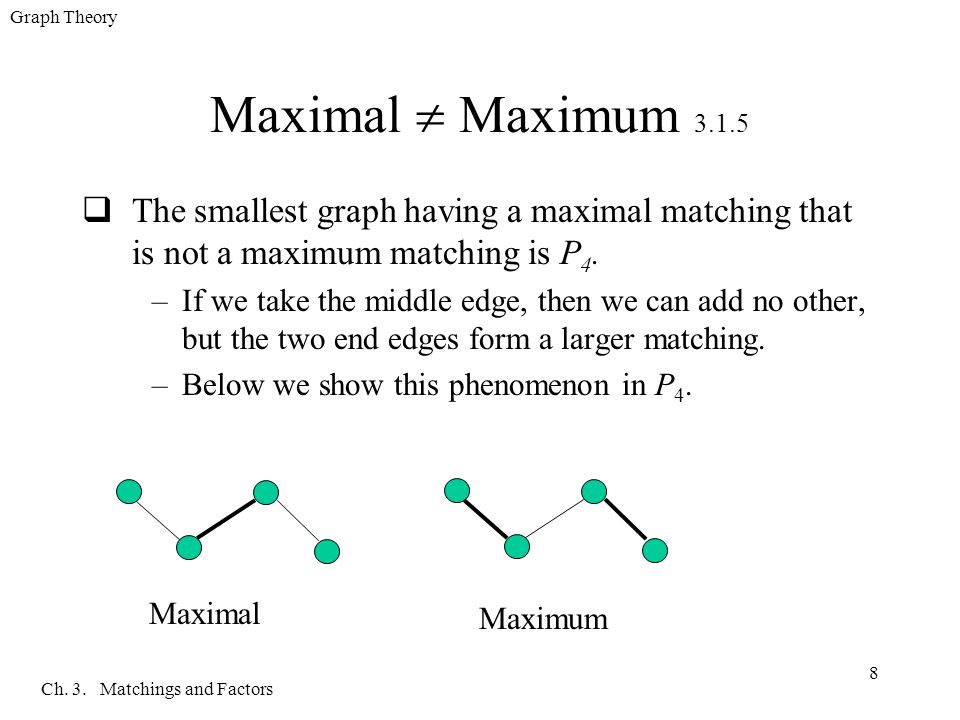
\includegraphics[scale=0.5]{slide_8.jpg}
    \\
    Consider, for example, a graph on 4 vertices and\\
    let $\pmb{X} = \{(2, 3)\}$ and $\pmb{Y} = \{(1, 2),(3, 4)\}$.\\
    Both $\pmb{X}$ and $\pmb{Y}$ are matchings, 
    but one cannot add an edge of $\pmb{Y}$ to $\pmb{X}$ and still have a matching.\\
    
    In graph above example I1 is satisfied\\
    But, I2 is not satisfied.\\
    Since I2 is not satisfied $\pmb{\mathcal{F}}$ is not a matroid here.\\
    So, any graph $\pmb{G}$ and $\pmb{\mathcal{F}}$ - family of independent sets in $\pmb{G}$, $\pmb{\mathcal{F}}$ is not necessarily a matroid.\\
    
    *Image credits - https://slideplayer.com/slide/10831654/
\end{solution}



\question Byteland, a country of area exactly $n$ square miles, has been divided by the government into
$n$ regions, each of area exactly one square mile. Meanwhile, the army of Byteland divided
its area into $n$ military zones, each of area again exactly one square mile. Show that one can
build   $n$ airports in Byteland, such that each region and each military zone contains (at least)
one airport. Furthermore, we can find locations where we should build such $n$ airports in
polynomial time.

\begin{solution}
    Construct the following bipartite graph: on one side there are regions of Byteland, on
the second side there are military zones, and a region R is adjacent to a zone Z if R∩Z = ∅.
Show that this graph satisfies the condition of Hall’s theorem and, consequently, contains
a perfect matching.\\\\
    
    The area of Byteland is $\pmb{n}$ $mi^2$ (i.e. $n$ square miles)\\
    Which is divided into $\pmb{n}$ small areas each of $1$ $mi^2$ by government and army each in their own way.\\
    This small areas are all polygons. (i.e. $\pmb{n}$ polygons)\\
    Let \textbf{map1} and \textbf{map2} be two map schemes by government and by army respectively.\\\\

    \textbf{To prove:-} $n$ airports can be built, such that each region and each military zone contains (at least) one airport.\\
    Lets place two maps \textbf{map1} and \textbf{map2} on top of another.\\
    we are looking for airports placed common through set of polygons both maps\\
    $\therefore$ We have to prove that an airport exit common on one polygon of one sheet and another polygon of the other sheet.\\
    i.e. Each airport is common to only two polygons(one from map1 other from map2).\\
    
    Construct a bipartite graph $\pmb{G} = \pmb{R} \cup \pmb{Z}$, $\pmb{R} = \{ r_1, r_2 . ., r_n \}$ and $\pmb{Z} = \{ z_1, z_2 . ., z_n \}$ with the bipartite sets being the $\pmb{n}$ polygons in either map.\\
    
    At this point, an idea is that the edges of the matching are the airports themselves.\\
    At micro-scale of this problem consider set $\mathbb{W}$ of polygons on $\pmb{map1}$ \\
    We need to prove that there are at least $|\mathbb{W}|$ polygons on the other map $\pmb{map2}$ that touch this subset $\mathbb{W}$.\\
    \\
    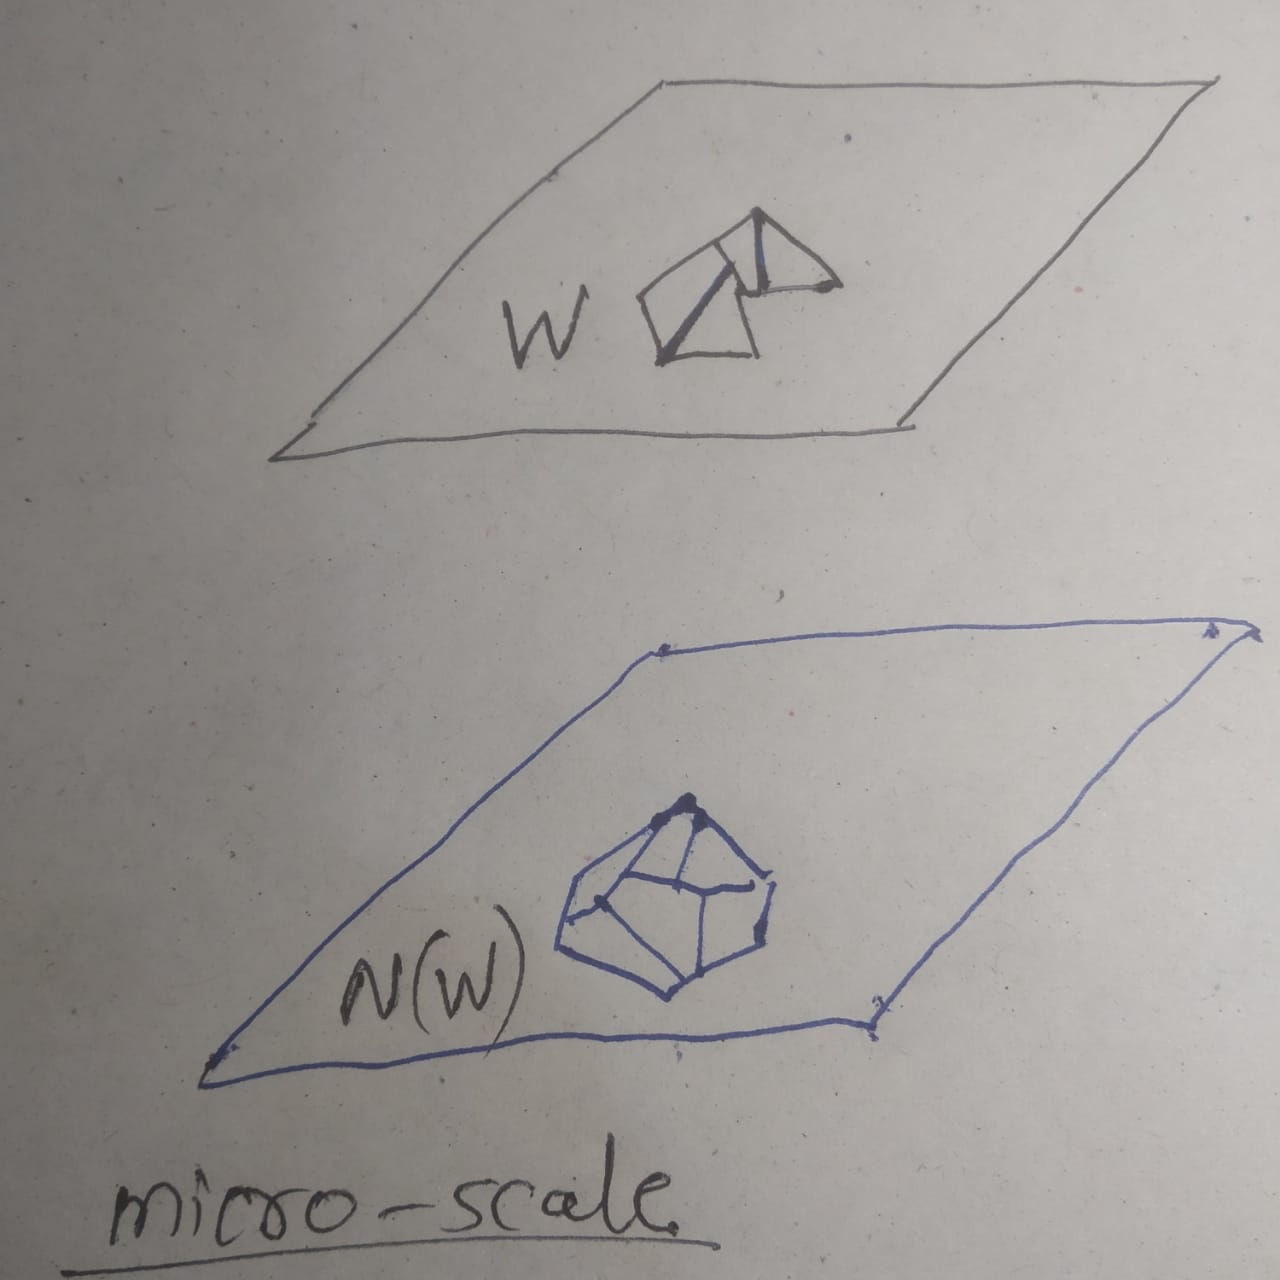
\includegraphics[scale=0.15]{fig1.jpeg} 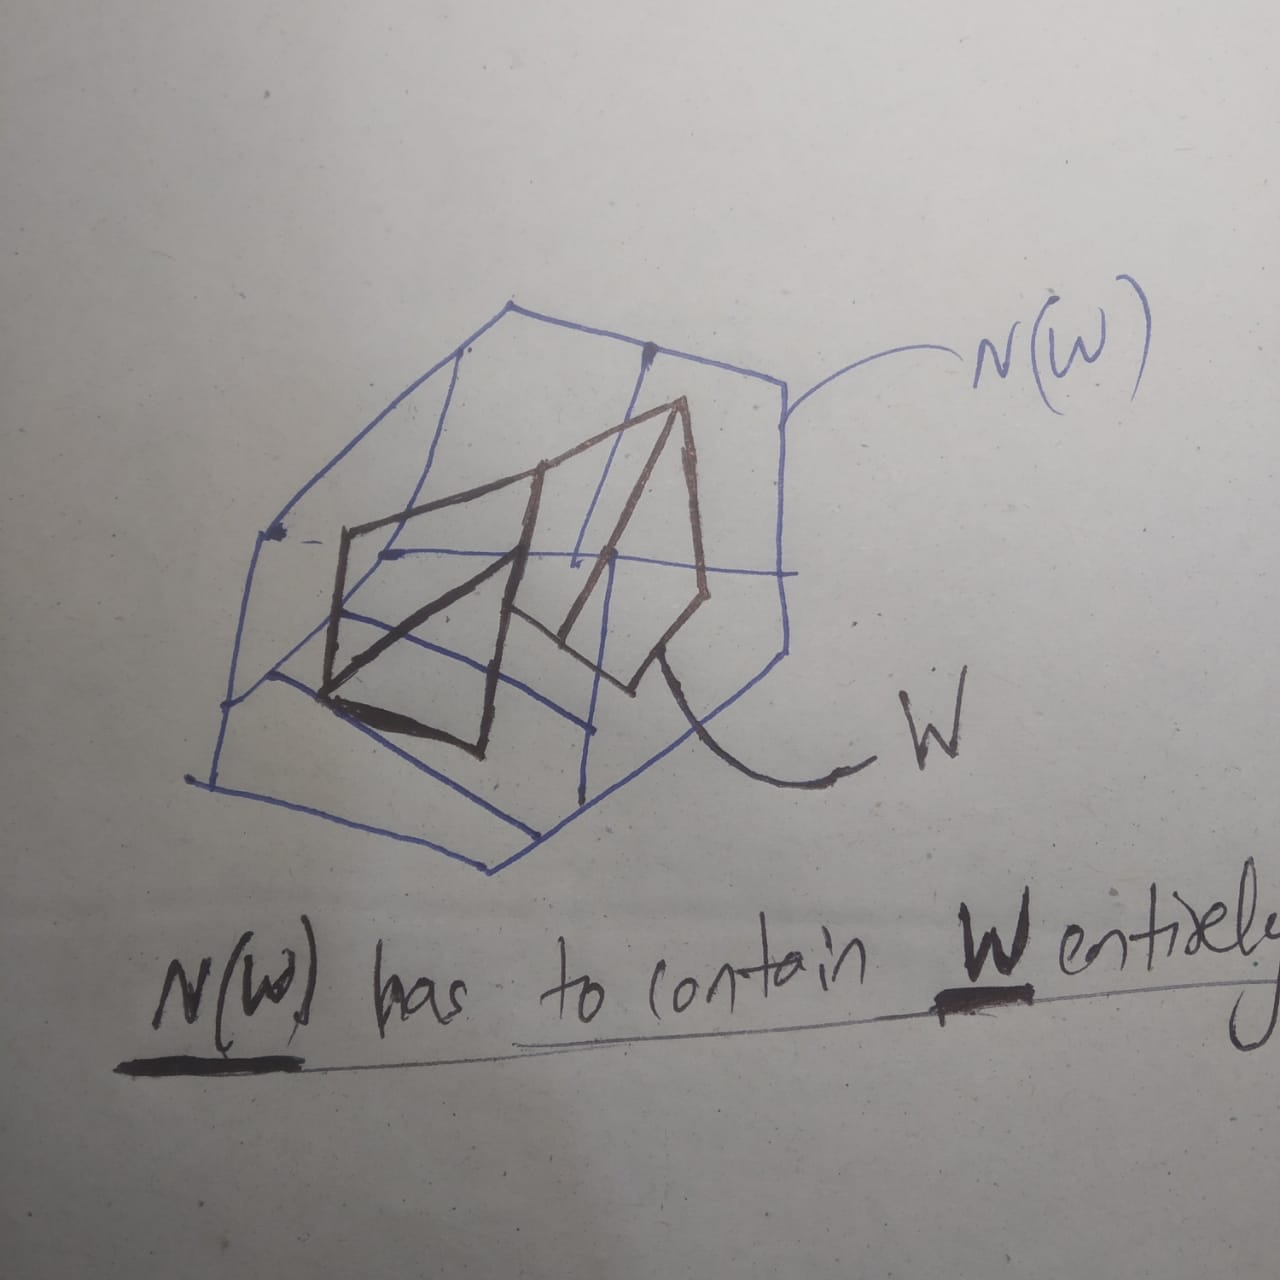
\includegraphics[scale=0.15]{fig2.jpeg}
    \\
    We try contradiction\\
    
    Take $\mathbb{W}$ and suppose that, say, less than $|\mathbb{W}|$ polygons intersect with it on the other map.\\
    We write $N(\mathbb{W})$ to denote the neighborhood of a set $\mathbb{W}$: the set of all vertices adjacent to some vertex of $\mathbb{W}$.\\
    i.e. assume $N(\mathbb{W}) < \mathbb{W}$\\
    Intuitively, this must mean that the polygons of $\mathbb{W}$ are “smaller” than those on $N(\mathbb{W})$, because they both occupy the same area\\
    We haven't used the information that each polygon have an area of $1$ $mi^2$\\\\
    $\implies$  The polygons of $\mathbb{W}$ have an area of exactly $|\mathbb{W}|$\\
    And the polygons of $N(\mathbb{W})$ have an area of exactly $|N(\mathbb{W})|$.\\
    But the region $N(\mathbb{W})$ has to contain the region of $\mathbb{W}$\\
    $\implies   \mathbb{W} \leq N(\mathbb{W})$ for any subset $\mathbb{W}$\\
    
    $\therefore$ by Hall’s theorem there exists a matching from one set of polygons to the other. We use this matching to find appropriate positions for the airports.

\end{solution}


\end{questions}
\end{document}
